\chapter{Публікація та оновлення відкритих даних}

\section{Вибір формату даних та конвертація даних з одного формату в інший}

Вибір формату даних залежить від способу збереження та інших факторів, проте в більшості випадків можна користуватись такими загальними правилами:

\begin{enumerate}
    \item \textbf{Неструктуровані текстові дані} (тексти законів, розпоряджень, довідкових даних):  
        \begin{itemize}
            \item Найкращий формат — Markdown або TXT.  
            \item Markdown підтримує додаткову розмітку (заголовки, абзаци, посилання, зображення тощо).  
            \item Вказуйте різновид Markdown.  
            \item HTML — гірший варіант, doc/docx, pdf/tiff — найгірші (окрім випадків, коли потрібна копія оригінального документу із підписом та печаткою).
        \end{itemize}
    \item \textbf{Табличні дані:}  
        \begin{itemize}
            \item Використовуйте формат CSV, у гіршому випадку — XLS/XLSX.
        \end{itemize}
    \item \textbf{Скани документів:}  
        \begin{itemize}
            \item Найкращий формат — TIFF, потім — PDF.
        \end{itemize}
    \item \textbf{Зображення:}  
        \begin{itemize}
            \item Обов'язкова роздільна здатність для OCR — не менше 300 dpi.
        \end{itemize}
    \item \textbf{Великі файли або групи файлів:}  
        \begin{itemize}
            \item Архівуйте у форматі ZIP/7Z.  
            \item Для файлів понад 4 ГБ — RAR.
        \end{itemize}
    \item \textbf{Дані, що змінюються постійно і формуються «на льоту»:}  
        \begin{itemize}
            \item Не обов'язково зберігати у вигляді файлів.  
            \item Достатньо надати доступ через Інтернет-адреси або API.  
            \item Рекомендовані формати для API: JSON/XML/RDF.
        \end{itemize}
    \item \textbf{Бінарні формати:}  
        \begin{itemize}
            \item Використовуйте лише за відсутності альтернативи.
        \end{itemize}
\end{enumerate}

Для конвертації даних існує багато інструментів: онлайн-сервіси, програмні засоби, бібліотеки. Зазвичай немає проблем з конвертацією між відкритими форматами. Проблеми можуть виникати з Word/PDF.

\textbf{Деякі програмні засоби для конвертації:}

\begin{itemize}
    \item Microsoft Word, Excel, Access
    \item Графічні формати та PDF: Adobe Photoshop, Acrobat Reader, Foxit PDF Reader, Paint.NET, Corel Draw
    \item Текстові дані: Notepad++
    \item Програмні засоби: SPSS, Microsoft Azure ML, Matlab
    \item Онлайн інструменти:  
        \begin{itemize}
            \item \href{http://konklone.io/json/}{JSON to CSV}  
            \item \href{http://www.convertcsv.com/csv-to-json.htm}{CSV to JSON}  
            \item \href{http://json2csharp.com/}{JSON to C\#}
        \end{itemize}
    \item Очищення HTML документів від Word-стилів: \href{https://word2cleanhtml.com/}{word2cleanhtml.com}
\end{itemize}

\section{Основні помилки при оприлюдненні відкритих даних}

\subsection{Чому Excel формат не є рекомендованим форматом?}

В Постанові дозволяється використовувати XLS/XLSX (Microsoft Excel). Проте Excel дозволяє додавати розширене форматування, об’єднані комірки, вбудовані об’єкти, макроси та формули, що ускладнює машинну обробку.

\textbf{Приклади неправильних Excel-документів:}

\begin{figure}[h]
    \centering
    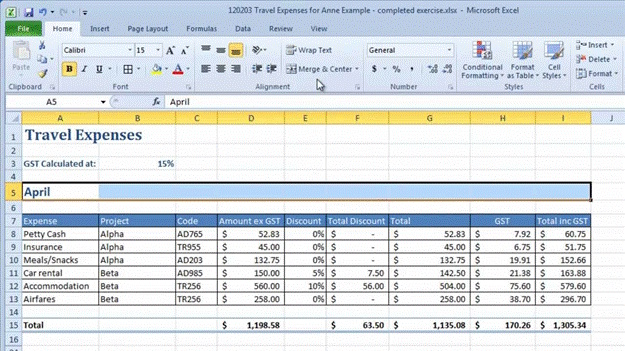
\includegraphics[width=0.5\textwidth]{images/004.jpg}
    \caption{Неправильний Excel 1}
\end{figure}

\begin{figure}[h]
    \centering
    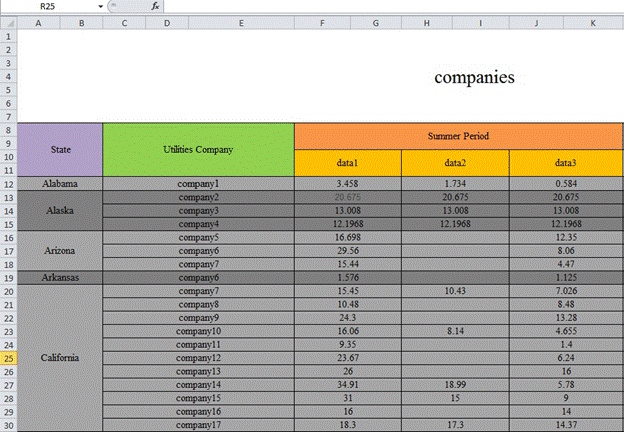
\includegraphics[width=0.5\textwidth]{images/005.jpg}
    \caption{Неправильний Excel 2}
\end{figure}

\textbf{Приклади правильних Excel-файлів:}

\begin{figure}[h]
    \centering
    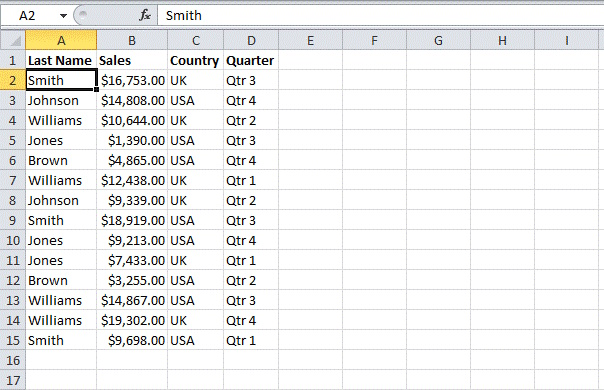
\includegraphics[width=0.5\textwidth]{images/006.jpg}
    \caption{Правильний Excel 1}
\end{figure}

\begin{figure}[h]
    \centering
    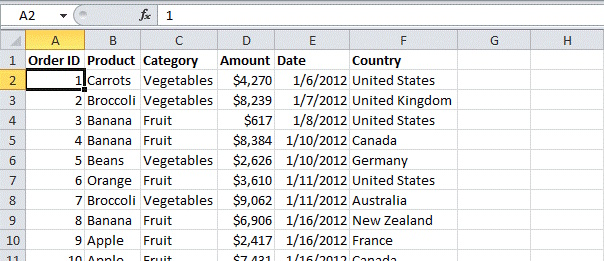
\includegraphics[width=0.5\textwidth]{images/007.jpg}
    \caption{Правильний Excel 2}
\end{figure}

Дані у правильному форматі легко експортувати у CSV.

\subsection{Оприлюднення занадто агрегованих даних}

\textbf{Очікується:}  
\begin{itemize}
    \item ділянка та її координати  
    \item дата ДТП  
    \item кількість постраждалих та тип ушкоджень  
    \item область (місто)  
    \item стан ділянки
\end{itemize}

\textbf{Неправильно:}  
\begin{itemize}
    \item лише кількість ДТП по областях
\end{itemize}

Розпорядники повинні публікувати детальну інформацію на рівні транзакцій, випадків або подій.

\section{Призначення відповідальних за розкриття даних}

Кожен розпорядник повинен визначити відповідальних осіб за аудит, обробку та публікацію відкритих даних. Вони повинні знати про доступні набори, формати, розміри, роботу з базами даних та користуватись порталом відкритих даних.

\section{Аудит наборів відкритих даних і пріоритетність їх публікації}

Публікація даних здійснюється поетапно, враховуючи:

\begin{enumerate}
    \item Потребу споживачів (за методикою моніторингу)
    \item Ступінь готовності (наявність даних, технічна готовність)
    \item Витрати на публікацію та підтримку
\end{enumerate}

\textbf{Фактори для формування реєстру:}

\begin{itemize}
    \item Публікуються дані без попередньої обробки
    \item Визначена відповідальна особа за кожен набір
    \item Встановлена періодичність оновлення
\end{itemize}

Реєстр затверджується органом і публікується на офіційному сайті.

\section{Підготовка даних до публікації}

\subsection{Кодування файлів}

Текст зберігається у вигляді числових значень згідно стандарту кодування.

\begin{itemize}
    \item \textbf{Windows-1251} — стандартне кодування для українських і російських версій Windows.  
        \href{https://uk.wikipedia.org/wiki/Windows-1251}{Детальніше}
    \item \textbf{UTF-8} — універсальне кодування, сумісне з ASCII.  
        \href{https://uk.wikipedia.org/wiki/UTF-8}{Детальніше}
\end{itemize}

Більшість державних органів використовують Windows-1251, що несумісне з іншими ОС. Перед публікацією на data.gov.ua переконайтесь, що файли збережені у UTF-8.

\textbf{Приклад проблем з кодуванням:}

\begin{figure}[h]
    \centering
    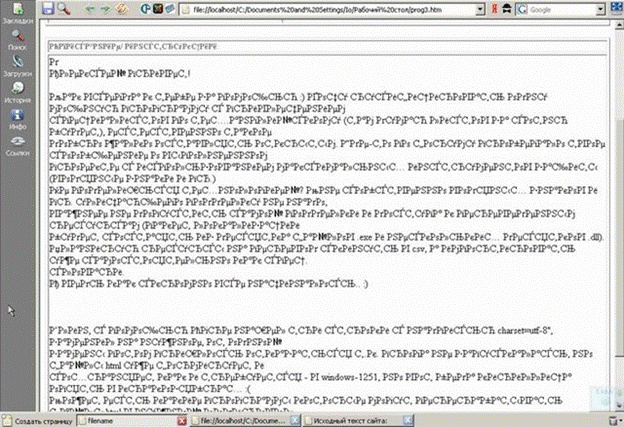
\includegraphics[width=0.5\textwidth]{images/008.jpg}
    \caption{Проблеми з кодуванням}
\end{figure}

\subsection{Один файл чи декілька?}

Якщо дані — реляційна база (MySQL, SQL Server, Oracle):

\begin{figure}[h]
    \centering
    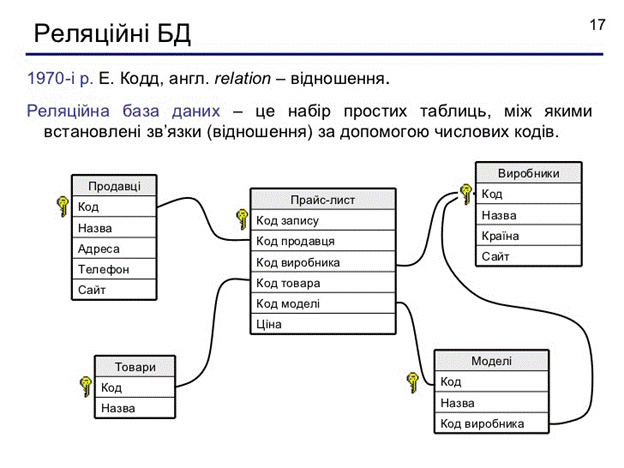
\includegraphics[width=0.5\textwidth]{images/009.jpg}
    \caption{Схема бази}
\end{figure}

\textbf{Приклад:}

\textit{Vendors (виробники)}

\begin{tabular}{|c|c|c|c|}
\hline
Id & Name      & Country & Website              \\
\hline
1  & Microsoft & USA     & http://microsoft.com \\
2  & Apple     & USA     & http://apple.com     \\
\hline
\end{tabular}

\textit{Models (моделі)}

\begin{tabular}{|c|c|c|}
\hline
Id & Name    & Vendor Code \\
\hline
1  & Surface & 1           \\
2  & iPhone  & 2           \\
\hline
\end{tabular}

\textbf{Варіант 1: Один файл}

\begin{verbatim}
models.csv:
Id;Name;Vendor;Country;Website
1;Surface;Microsoft;USA;http://microsoft.com
2;iPhone;Apple;USA;http://apple.com
\end{verbatim}

\textbf{Варіант 2: Два файли}

\begin{verbatim}
vendors.csv:
Id;Name;Country;Website
1;Microsoft;USA;http://microsoft.com
2;Apple;USA;http://apple.com

models.csv:
Id;Name;VendorId
1;Surface;1
2;iPhone;2
\end{verbatim}

\textbf{Порівняння:}

\begin{tabular}{|l|l|l|}
\hline
Критерій                           & Один файл                                                & Багато файлів                        \\
\hline
Збитковість даних                   & Велика                                                  & Мала                                 \\
Фінальний розмір                    & Більший                                                 & Менший                               \\
Перевірка на цілісність             & Складна                                                 & Проста                               \\
Готовність до використання через API & Погана                                                  & Хороша                               \\
Кількість запитів                   & Один (перевага для малих файлів)                        & Багато                               \\
\hline
\end{tabular}

Другий варіант доцільніший.

\subsection{Деперсоніфікація даних}

Згідно \href{http://zakon3.rada.gov.ua/laws/show/2297-17}{Закону “Про захист персональних даних”}, персональні дані — будь-які відомості, за якими ідентифікується особа. Такі дані мають бути деперсоніфіковані перед публікацією.

\textbf{Приклад:}

\textit{Початкові дані:}

\begin{tabular}{|l|l|l|l|}
\hline
ПІП         & Місто & Телефон      & Група крові \\
\hline
Іванов І.І. & Київ  & 011 111 11 11& A(I)+       \\
Петров П.П. & Одеса & 011 111 11 12& B(II)-      \\
\hline
\end{tabular}

\textit{Кроводачі:}

\begin{tabular}{|l|l|l|}
\hline
ПІП         & Центр    & Дата       \\
\hline
Іванов І.І. & Охматдит & 01.01.2016 \\
Петров П.П. & Охматдит & 01.02.2016 \\
\hline
\end{tabular}

\textit{Після деперсоніфікації:}

\begin{tabular}{|l|l|l|}
\hline
ПІП & Місто & Група крові \\
\hline
1   & Київ  & A(I)+       \\
2   & Одеса & B(II)-      \\
\hline
\end{tabular}

\textit{Кроводачі:}

\begin{tabular}{|l|l|l|}
\hline
ПІП & Центр    & Дата       \\
\hline
1   & Охматдит & 01.01.2016 \\
2   & Охматдит & 01.02.2016 \\
\hline
\end{tabular}

\subsection{Архівація наборів даних}

Архівація зменшує розмір файлів і трафік. Текстові дані стискаються до 90\%, Word/Excel/PDF — на 10-60\%, зображення — майже не стискаються.

\textbf{Архівувати потрібно:}

\begin{itemize}
    \item історичні дані
    \item файли понад 50 МБ
    \item застарілі версії наборів
    \item багатотомні набори
\end{itemize}

\textbf{Рекомендовані формати:} zip/7z/tar.  
\textbf{Рекомендована програма:} \href{http://7-zip.org.ua/}{7-zip}

\subsection{Публікація даних, що мають періодичність}

Набори поділяються на:

\begin{itemize}
    \item \textbf{Частопубліковані} (оновлення частіше 1 раз на тиждень)
    \item \textbf{Рідкопубліковані} (рідше 1 раз на тиждень)
\end{itemize}

В паспорті набору вказується дата останнього оновлення.

\textbf{Частота оновлень:}

\begin{itemize}
    \item Часто: більше одного разу в день, щодня, щотижня
    \item Рідко: щомісяця, щокварталу, кожні півроку, щороку, по мірі змін
\end{itemize}

\textbf{Приклади іменування файлів:}

\begin{itemize}
    \item За датою: \texttt{exchange\_20160101.csv}
    \item За валютою: \texttt{exchange\_usd.csv}
\end{itemize}

Якщо дані змінюються постійно — організуйте доступ через API.

\subsection{Публікація схожих даних з різними структурами}

Якщо структура схожа — об'єднайте всі поля, відсутні дані залишайте порожніми.

\textbf{Приклад:}

\begin{verbatim}
A1,A2,A3,A4
1,1,1,1

A1,A2,A3,A5
2,2,2,2
\end{verbatim}

\textbf{Фінальний файл:}

\begin{verbatim}
A1,A2,A3,A4,A5
1,1,1,1,
2,2,2,,2
\end{verbatim}

Якщо структура відрізняється значно — розглядайте файли окремо.

\subsection{Публікація даних у вигляді API та робота з великими обсягами}

Два основних способи доступу:

\begin{itemize}
    \item \textbf{Data Hub} — для рідко змінюваних даних
    \item \textbf{API} — для оперативних запитів
\end{itemize}

Рекомендується використовувати \href{http://www.odata.org/}{OData} для API.

В описі набору вказуйте тип даних, посилання на документацію, умови доступу, обмеження, формати, підтримку OData.

\subsection{Канали розповсюдження відкритих даних}

\begin{enumerate}
    \item Через сайт \href{https://data.gov.ua}{data.gov.ua}
    \item Через сайти місцевих органів самоврядування
    \item За допомогою API
    \item Через ftp-сервер
    \item Через BitTorrent
\end{enumerate}
